\subsection*{7(a)}
We can first rearrange the constraints 2 and 3 into the following form by moving elements on the right handside to the left and multiplying constraints 2 by $-1$.
\begin{equation*}
\begin{aligned}
- w^Tx_i - b + 1 - \xi_i &\leq 0\\ \mbox{ if } y_i = 1
w^Tx_i + b + 1 - \xi_i &\leq 0\\ \mbox{ if } y_i = -1
\end{aligned} 
\end{equation*}
Through observing the inequalities, we notice that the only difference is the element $w^Tx_i$ which has a different sign that could be change by the values of $y_i$. This allows us to combine both inequalities into the following constraint.
\begin{equation*}
- y_i(w^Tx_i + b) + 1 - \xi_i \leq = 0
\end{equation*}

\subsection*{7(b)}
The Lagrangian for our optimization problem is as following:
\begin{equation*}
L ([w\;0\;\xi]^T, \alpha, \beta) = \frac{1}{2}||w||^2 + C \sum_{i=1}^l \xi_i + \sum_{i=1}^l \alpha_ig_i([w\;b\;\xi]^T) - \sum_{i=1}^l \beta_i \xi_i
\end{equation*}

\subsection*{7(c)}
Following is the steps to minimize the Lagrangian which is ther primal form of the SVM. Here's the original Lagrangian.
\begin{equation}\label{ori-l}
L ([w\;0\;\xi]^T, \alpha, \beta) = \frac{1}{2}||w||^2 + C \sum_{i=1}^l \xi_i + \sum_{i=1}^l \alpha_i(- y_i(w^Tx_i + b) + 1 - \xi_i) - \sum_{i=1}^l \beta_i \xi_i
\end{equation}
First we, find the partial of $w$,$b$ and $\xi_i$. Following are the partials follow by setting them to 0.\\
Finding partial of $w$
\begin{equation}\label{wpartial}
\begin{aligned}
\frac{\partial}{\partial w} &= \frac{2}{2} w - \sum_{i=1}^l(\alpha_i y_i x_i) = 0\\
w &= \sum_{i=1}^l(\alpha_i y_i x_i)
\end{aligned}
\end{equation}
Finding the partial of $b$.
\begin{equation}\label{bpartial}
\begin{aligned}
\frac{\partial}{\partial b} &= -\sum_{i=1}^l(\alpha_i y_i) = 0\\
\sum_{i=1}^l(\alpha_i y_i) &= 0\\
\end{aligned}
\end{equation}
Finding the partial of $xi_i$.
\begin{equation}\label{xipartial}
\begin{aligned}
\frac{\partial}{\partial \xi_i} &= C - \sum_{i=1}^l(\alpha_i) - \sum_{i=1}^l(\beta_i) = 0\\
C &= \sum_{i=1}^l(\alpha_i) + \sum_{i=1}^l(\beta_i)
\end{aligned}
\end{equation}\tabularnewline
Now we insert equations \ref{wpartial}, \ref{xipartial} in equation \ref{ori-l}.
\begin{equation}
\begin{aligned}
L &= \frac{1}{2}(\sum_{i=1}^l(\alpha_i y_i x_i))^2 + (\sum_{i=1}^l(\alpha_i) + \sum_{i=1}^l(\beta_i))\sum_{i=1}^l \xi_i + \sum_{i=1}^l \alpha_i(- y_i((\sum_{j=1}^l(\alpha_j y_j x_j))x_i + b) + 1 - \xi_i) - \sum_{i=1}^l \beta_i \xi_i\\
L &= \frac{1}{2}(\sum_{i=1}^l\sum_{j=1}^l(\alpha_i \alpha_j y_i y_j x_j^T x_i)) + \sum_{i=1}^l(\alpha_i \xi_i) + \sum_{i=1}^l(\beta_i \xi_i) + \sum_{i=1}^l(\alpha_i \alpha_j y_i y_j x_j^T x_i))\\
&- b \sum_{i=1}^l(\alpha_i y_i) + \sum_{i=1}^l(\alpha_i) - \sum_{i=1}^l(\alpha_i \xi_i) - \sum_{i=1}^l \beta_i \xi_i\\
L &= \sum_{i=1}^l(\alpha_i) - \frac{1}{2}(\sum_{i=1}^l\sum_{j=1}^l(\alpha_i \alpha_j y_i y_j x_j^T x_i)) - b \sum_{i=1}^l(\alpha_i y_i)\\
\end{aligned}
\end{equation}
By applying equation \ref{bpartial} in the previous equation, we can derive the final form
\begin{equation}\label{final-eq}
L^*(\alpha) = \sum_{i=1}^l(\alpha_i) - \frac{1}{2}(\sum_{i=1}^l\sum_{j=1}^l(\alpha_i \alpha_j y_i y_j x_j^T x_i))\\
\end{equation}

\subsection*{7(d)}
As we want to write the equation in terms of $H$ and $f$ such that $L^*(\alpha) = \frac{1}{2} \alpha^TH\alpha + f^T\alpha$. By looking at equation \ref{final-eq}, we see a similar structure between them. For the first part $\frac{1}{2} \alpha^TH\alpha $
\begin{equation*}
\begin{aligned}
\frac{1}{2}\alpha^TH\alpha &= \frac{1}{2}(\sum_{i=1}^l\sum_{j=1}^l(\alpha_i \alpha_j y_i y_j x_j^T x_i))\\
H &= (\sum_{i=1}^l\sum_{j=1}^l(y_i y_j x_j^T x_i))
\end{aligned}
\end{equation*}
For second part $f^T\alpha$
\begin{equation*}
\begin{aligned}
f^T\alpha &= \sum_{i=1}^l(\alpha_i)\\
f^T &= [1,1,.....1]
\end{aligned}
\end{equation*}

\subsection*{7(e)(iii)}
Following is the table showing the accuracy of my algorithm on a 10-fold cross validation run.\\
\begin{centering}
\begin{tabular}{|c|c|c|c|c|c|c|c|}
\hline
k & correct P & wrongly label & P detection \% & correct N & wrongly label & N detection \% & total accuracy \\ \hline
1 & 49 & 0 & 0.326667 & 104 & 101 & 1 & 0.602362 \\ \hline 
2 & 70 & 0 & 0.526316 & 120 & 63 & 1 &0.750988 \\ \hline 
3 & 68 & 0 & 0.539683 & 128 & 58 & 1 &0.771654 \\ \hline 
4 & 63 & 0 & 0.463235 & 117 & 73 & 1 &0.711462 \\ \hline 
5 & 52 & 0 & 0.382353 & 118 & 84 & 1 &0.669291 \\ \hline 
6 & 75 & 0 & 0.539568 & 114 & 64 & 1 &0.747036 \\ \hline 
7 & 70 & 0 & 0.514706 & 117 & 66 & 1 &0.739130 \\ \hline 
8 & 75 & 0 & 0.547445 & 116 & 62 & 1 &0.754941 \\ \hline 
9 & 65 & 0 & 0.481481 & 118 & 70 & 1 &0.723320 \\ \hline 
10 & 78 & 0 & 0.609375 & 126 & 50 & 1 &0.803150 \\ \hline 
\end{tabular}
\end{centering}
One interesting observation is that the SVM overclassifies the negative(the hand writing zero). It has 100\% accuracy on classifying that hand writing but also falsely detect multiple ones in the process.
\subsection*{7(e)(iv)}
\begin{figure}[H]
\centering
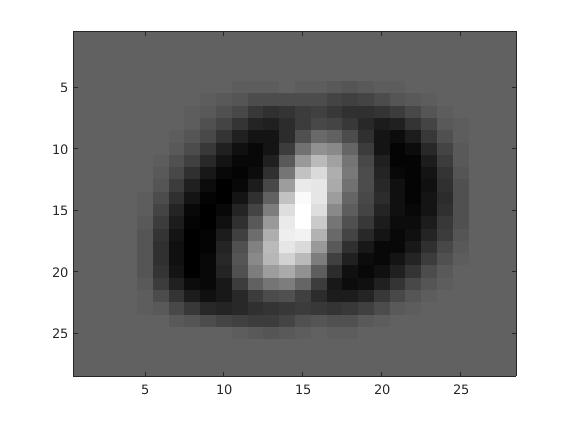
\includegraphics[width=6.5in]{figures/q7-6.jpg}
\caption{plot of weight function}
\end{figure}
The weight functions shows what the algorithm learns. It assigns positive number when it detects features in the middle and assigns negative values to features around in the circle. One possibility that zero has a higher accuracy than one is that most of the zero's feature space does not overlap with ones and it also has a larger area. Where as one, it relies on the middle and also the edge which it shares with zero(you can see the slight discoloration on those are compare to the side of the zero). The selection of the feature space is really important and the larger size of zero in the feature space has skewed the result towards it.
